\hypertarget{specification-of-the-thirteen-process-parameters}{%
\chapter{Specification of the Thirteen Process Parameters}\label{specification-of-the-thirteen-process-parameters}}

This appendix gives the complete specification of the machine-native process parameters that constitute the feature vector used throughout this thesis. Column names are reproduced exactly as they appear in the dataset and in the implementation, because several use the machine manufacturer's abbreviation codes and consistency between thesis and code is required for reproducibility.

\hypertarget{a.1-parameter-definitions-and-descriptive-statistics}{%
\section{A.1 Parameter Definitions and Descriptive Statistics}\label{a.1-parameter-definitions-and-descriptive-statistics}}

\textbf{Table A.1.} Full specification of the thirteen process parameters. Units and physical descriptions from Polenta et al.~{[}5{]}, Table 1. Minimum and maximum are the observed extremes over the full raw dataset (n = 1,451); mean and standard deviation are computed over the same population. Source: \texttt{config/constraints.yaml} (auto-generated from \texttt{data/raw/raw\_data.csv}) and \texttt{thesis\_assets/data/feature\_specification.json}.

\begin{longtable}[]{@{}
  >{\raggedright\arraybackslash}p{(\columnwidth - 16\tabcolsep) * \real{0.1111}}
  >{\raggedright\arraybackslash}p{(\columnwidth - 16\tabcolsep) * \real{0.1111}}
  >{\raggedright\arraybackslash}p{(\columnwidth - 16\tabcolsep) * \real{0.1111}}
  >{\raggedright\arraybackslash}p{(\columnwidth - 16\tabcolsep) * \real{0.1111}}
  >{\raggedright\arraybackslash}p{(\columnwidth - 16\tabcolsep) * \real{0.1111}}
  >{\raggedright\arraybackslash}p{(\columnwidth - 16\tabcolsep) * \real{0.1111}}
  >{\raggedright\arraybackslash}p{(\columnwidth - 16\tabcolsep) * \real{0.1111}}
  >{\raggedright\arraybackslash}p{(\columnwidth - 16\tabcolsep) * \real{0.1111}}
  >{\raggedright\arraybackslash}p{(\columnwidth - 16\tabcolsep) * \real{0.1111}}@{}}
\toprule\noalign{}
\begin{minipage}[b]{\linewidth}\raggedright
\#
\end{minipage} & \begin{minipage}[b]{\linewidth}\raggedright
Parameter (dataset column)
\end{minipage} & \begin{minipage}[b]{\linewidth}\raggedright
Unit
\end{minipage} & \begin{minipage}[b]{\linewidth}\raggedright
Physical meaning
\end{minipage} & \begin{minipage}[b]{\linewidth}\raggedright
Process stage
\end{minipage} & \begin{minipage}[b]{\linewidth}\raggedright
Min
\end{minipage} & \begin{minipage}[b]{\linewidth}\raggedright
Max
\end{minipage} & \begin{minipage}[b]{\linewidth}\raggedright
Mean
\end{minipage} & \begin{minipage}[b]{\linewidth}\raggedright
Std
\end{minipage} \\
\midrule\noalign{}
\endhead
\bottomrule\noalign{}
\endlastfoot
1 & Melt temperature & °C & Temperature of the polymer before injection into the mold & Plasticizing & 81.747 & 155.032 & 106.892 & 5.6158 \\
2 & Mold temperature & °C & Temperature of the mold & Cooling & 78.409 & 82.159 & 81.326 & 0.4288 \\
3 & time\_to\_fill & s & Time taken to fill the mold cavity & Injection & 6.084 & 11.232 & 7.459 & 1.6881 \\
4 & ZDx -- Plasticizing time & s & Time to plasticize the material for one shot & Plasticizing & 2.780 & 6.610 & 3.2342 & 0.3432 \\
5 & ZUx -- Cycle time & s & Time to complete the entire cycle for one product & Whole cycle & 74.780 & 75.790 & 75.2188 & 0.4328 \\
6 & SKx -- Closing force & N † & Closing force applied to the mold & Clamping & 876.7 & 930.6 & 901.9748 & 11.0982 \\
7 & SKs -- Clamping force peak value & N † & Peak value of the mold closing force & Clamping & 894.8 & 946.5 & 919.3518 & 10.7800 \\
8 & Ms -- Torque peak value current cycle & N·m & Peak torque on the injection screw & Plasticizing & 94.2 & 130.3 & 116.7167 & 5.0291 \\
9 & Mm -- Torque mean value current cycle & N·m & Mean torque on the injection screw & Plasticizing & 76.5 & 114.9 & 104.1639 & 4.8022 \\
10 & APSs -- Specific back pressure peak value & bar & Peak resistance against the injection screw & Plasticizing & 144.8 & 150.5 & 146.2300 & 0.8049 \\
11 & APVs -- Specific injection pressure peak value & bar & Peak injection pressure & Injection & 780.5 & 943.0 & 900.9728 & 25.5192 \\
12 & CPn -- Screw position at the end of hold pressure & cm & Screw position at the end of the holding phase & Packing & 8.33 & 9.06 & 8.8089 & 0.0972 \\
13 & SVo -- Shot volume & cm³ & Volume of material injected & Injection & 18.51 & 19.23 & 18.7563 & 0.0955 \\
\end{longtable}

† See the unit-convention note in §A.3.

Per-split medians and quartiles are exported to \texttt{thesis\_assets/data/feature\_specification.json}; the 13 × 13 Pearson correlation matrix computed on the training split is exported to \texttt{thesis\_assets/data/correlation\_matrix.csv} and rendered as a heatmap in \texttt{thesis\_assets/figures/ch3/fig\_ch3\_correlation\_heatmap}.

\begin{figure}[htbp]
\centering
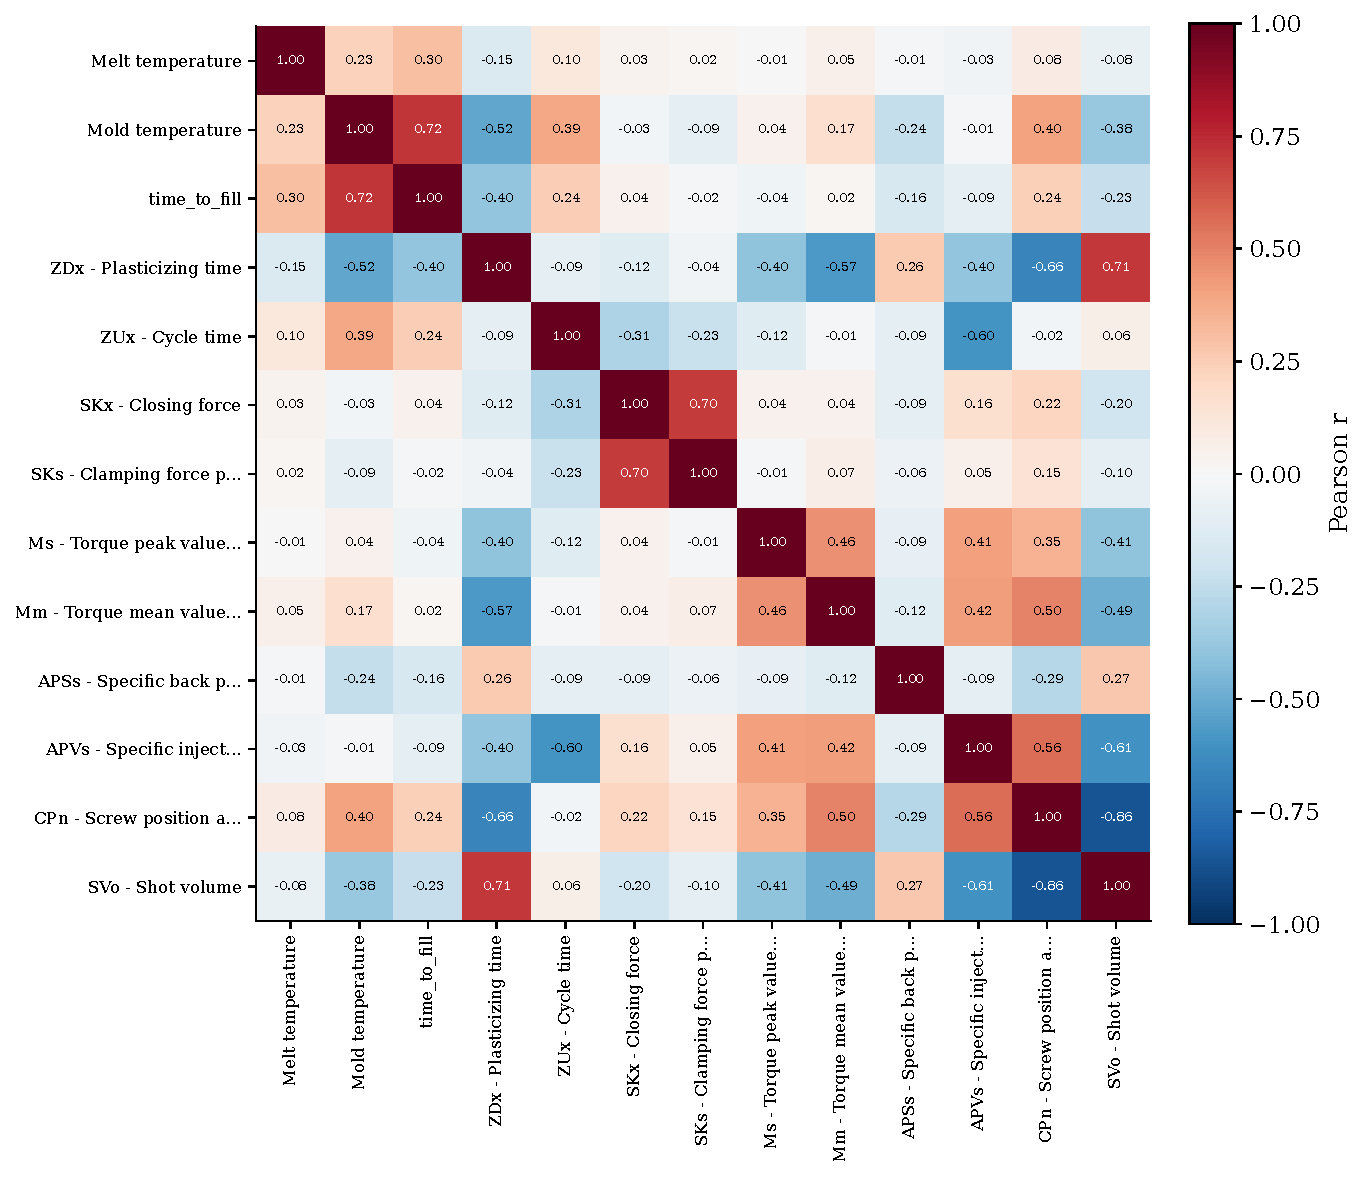
\includegraphics[width=0.75\textwidth]{figures/ch3/fig_ch3_correlation_heatmap.pdf}
\caption{Pearson correlation matrix of the 13 process parameters, training split. Source: \texttt{thesis\_assets/data/correlation\_matrix.csv}, \texttt{thesis\_assets/figures/ch3/fig\_ch3\_correlation\_heatmap}.}
\label{fig:ch3-correlation-heatmap}
\end{figure}

\hypertarget{a.2-setpoint-versus-measured-outcome-classification}{%
\section{A.2 Setpoint versus Measured-Outcome Classification}\label{a.2-setpoint-versus-measured-outcome-classification}}

Section 5.1.3 established a distinction that has no consequence for classification but a substantial one for counterfactual recommendation: some of these quantities are values an operator sets on the machine controller, while others are values the machine measures as a consequence of the cycle. A recommendation to change a measured outcome is not directly executable, because there is no field on the control panel corresponding to it.

\textbf{Table A.2.} Provisional classification of the thirteen parameters by controllability. \textbf{This classification is inferred from the parameter descriptions and from general injection molding practice; it has not been verified against the Engel E-MAC 310/100 controller documentation and should be confirmed before being relied upon.} It is the basis of the setpoint-restriction experiment proposed in §6.4 (F2).

\begin{longtable}[]{@{}
  >{\raggedright\arraybackslash}p{(\columnwidth - 4\tabcolsep) * \real{0.3333}}
  >{\raggedright\arraybackslash}p{(\columnwidth - 4\tabcolsep) * \real{0.3333}}
  >{\raggedright\arraybackslash}p{(\columnwidth - 4\tabcolsep) * \real{0.3333}}@{}}
\toprule\noalign{}
\begin{minipage}[b]{\linewidth}\raggedright
Parameter
\end{minipage} & \begin{minipage}[b]{\linewidth}\raggedright
Classification
\end{minipage} & \begin{minipage}[b]{\linewidth}\raggedright
Basis
\end{minipage} \\
\midrule\noalign{}
\endhead
\bottomrule\noalign{}
\endlastfoot
Melt temperature & Setpoint & Barrel zone temperature is directly set \\
Mold temperature & Setpoint & Mold temperature controller setpoint \\
SKx -- Closing force & Setpoint & Clamp force is configured per job \\
SVo -- Shot volume & Setpoint & Shot size / metering stroke is configured \\
time\_to\_fill & Partly derived & Consequence of the injection speed profile; measured per cycle \\
ZDx -- Plasticizing time & Derived & Consequence of screw rotation speed and back pressure \\
ZUx -- Cycle time & Derived & Aggregate of injection, hold, cooling and mold movement times \\
SKs -- Clamping force peak value & Measured & Peak of the realised clamping force \\
Ms -- Torque peak value & Measured & Peak screw torque during plasticizing \\
Mm -- Torque mean value & Measured & Mean screw torque during plasticizing \\
APSs -- Specific back pressure peak & Measured & Peak of the realised back pressure \\
APVs -- Specific injection pressure peak & Measured & Peak of the realised injection pressure \\
CPn -- Screw position at end of hold & Measured & Realised screw position at hold-pressure cut-off \\
\end{longtable}

Four parameters are cleanly settable; the remaining nine are wholly or partly consequences of the cycle. The three parameters that dominate the SHAP ranking (§4.3.1) --- cycle time, plasticizing time and filling time --- all fall in the derived group.

\hypertarget{a.3-note-on-unit-conventions}{%
\section{A.3 Note on Unit Conventions}\label{a.3-note-on-unit-conventions}}

Two of the recorded parameters carry values that appear inconsistent with typical engineering magnitudes for the units stated in the source publication. This is recorded here as a data-provenance observation, not as a claimed error in the source.

\textbf{Closing and clamping force.} These are stated in newtons and recorded at approximately 900--950. The machine identified in the source publication is an Engel E-MAC 310/100, whose designation indicates a clamping force in the region of 100 metric tonnes, or approximately 1,000 kN. A recorded value of 908 is therefore consistent with \textbf{kilonewtons} rather than newtons --- placing the process at roughly 90\% of the machine's rated clamping force, which is an unremarkable operating point.

\textbf{Melt temperature.} This is stated in degrees Celsius and recorded with a mean of 106.9 °C. Melt temperatures for optical thermoplastics used in road lenses are typically in the range 220--300 °C. The recorded quantity may therefore be a specific barrel zone, a controller-internal scaled value, or a differential rather than an absolute melt temperature.

\textbf{Consequence for this work: none, and this is worth being precise about.} Every method in this thesis operates on the values exactly as recorded, and every recommendation is expressed in the same units and on the same scale as the input. The counterfactual engine's bound enforcement (§3.6.5) clips to the observed range of the recorded values, so no recommendation departs from the range the machine was actually operated at, whatever the units of that range denote.

\textbf{Consequence for deployment: material.} Before any recommendation produced by this framework is transferred to a physical machine, the unit convention of every parameter must be confirmed against the machine's own controller documentation. A recommendation to reduce closing force by 4.18 units is a 0.46\% adjustment if the unit is kN and a physically meaningless one if it is N. This is recorded as a precondition of the physical validation trial specified in §6.4 (F1).

\hypertarget{a.4-feature-name-consistency}{%
\section{A.4 Feature Name Consistency}\label{a.4-feature-name-consistency}}

The exact feature-name strings below are asserted in the test suite (\texttt{tests/test\_data.py}, \texttt{EXPECTED\_FEATURES}) and must match the dataset column headers, the persisted \texttt{feature\_names.pkl} artefact, and every reference in the source code. Any divergence causes a key-lookup failure at run time rather than a silent error.

\begin{verbatim}
Melt temperature
Mold temperature
time_to_fill
ZDx - Plasticizing time
ZUx - Cycle time
SKx - Closing force
SKs - Clamping force peak value
Ms - Torque peak value current cycle
Mm - Torque mean value current cycle
APSs - Specific back pressure peak value
APVs - Specific injection pressure peak value
CPn - Screw position at the end of hold pressure
SVo - Shot volume
\end{verbatim}

Note the inconsistent naming convention inherited from the source dataset: \texttt{time\_to\_fill} uses lowercase snake case while the remaining twelve use the machine's abbreviation code followed by a hyphen-separated description, and two use plain English. The names are reproduced unmodified rather than normalised, so that the dataset as published and the dataset as consumed remain byte-identical.
